% DO NOT COMPILE THIS FILE DIRECTLY!
% This is included by the other .tex files.

\begin{frame}[t,plain]
\titlepage
\end{frame}

\begin{frame}[t]{Motivating Problem I}
\begin{itemize}
\item How many sinusoids are in this data?
\item Also, what are their periods, amplitudes and phases?
\end{itemize}
\begin{center}
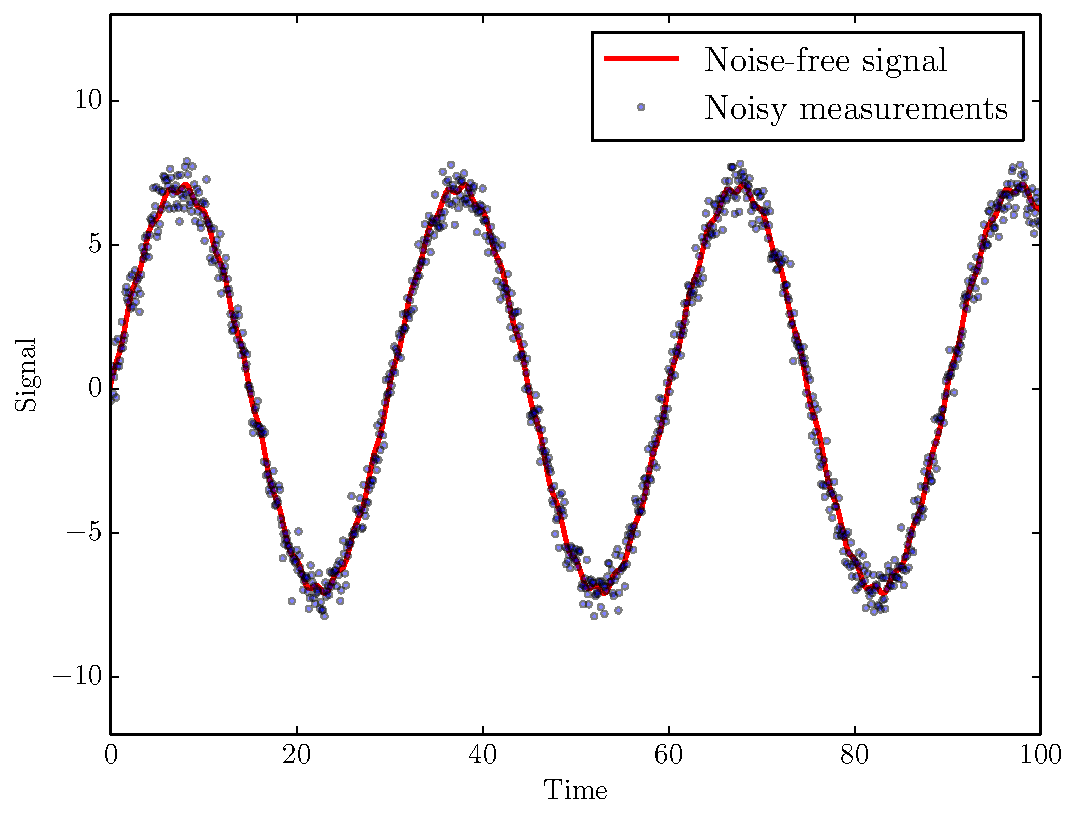
\includegraphics[scale=0.35]{sinewave_data.pdf}
\end{center}
\end{frame}

\begin{frame}[t]{Motivating Problem I}
Problems like this arise both inside and outside of astronomy,
for example:
\vspace{20pt}
\begin{itemize}
\item Asteroseismology
\item Extrasolar planets (radial velocity technique)
\end{itemize}
\end{frame}

\begin{frame}[t]{Motivating Problem II}
\begin{itemize}
\item How many stars are in these images?
\item Also, what are their positions, fluxes, etc?
\end{itemize}
\begin{center}
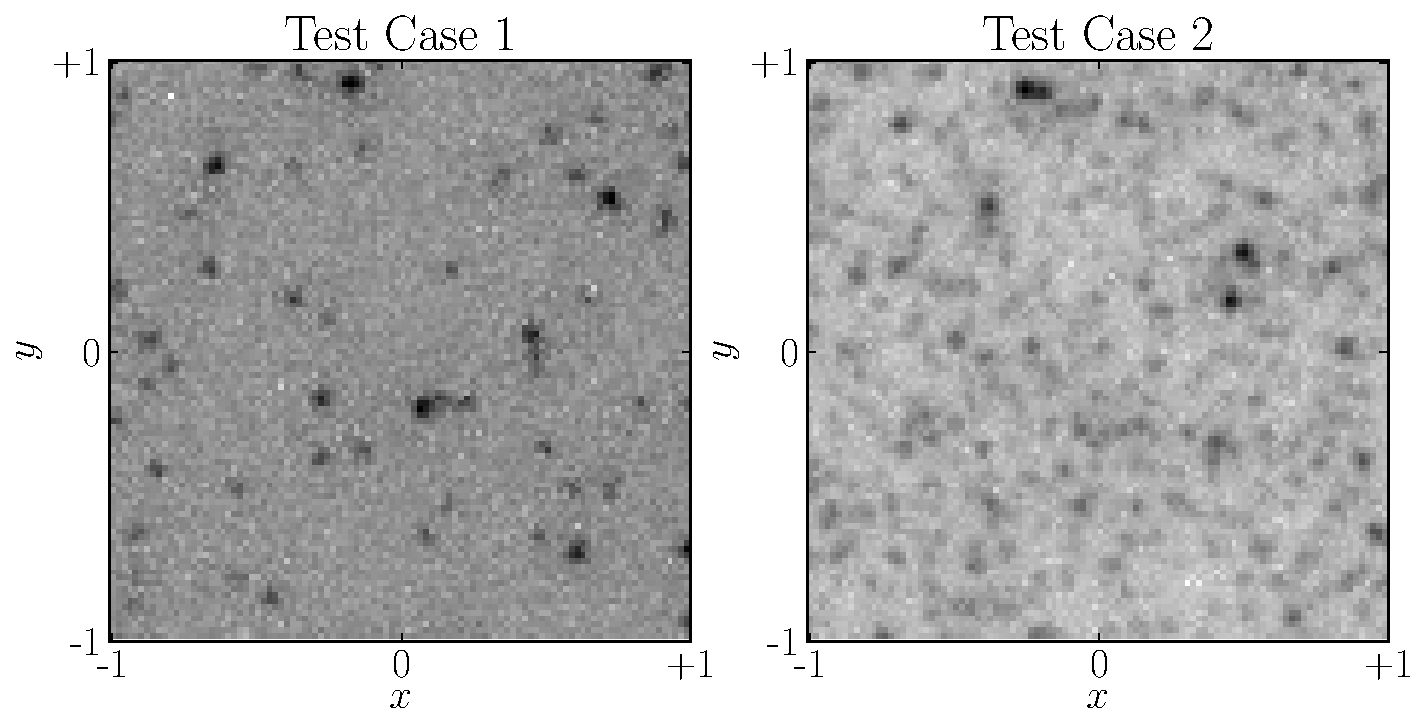
\includegraphics[scale=0.35]{test_cases.pdf}
\end{center}
\end{frame}

\begin{frame}[t]{Motivating Problem II}
This is a fundamental task in astronomy!
\end{frame}


\begin{frame}[t]{Bayesian Inference 101}
Bayesian Inference is a unified framework for solving inference problems.
We need the following ingredients:

\begin{itemize}
\setlength{\itemsep}{20pt}
\item A {\bf hypothesis space} describing the set of possible answers to our
question (``parameter space'' in fitting is the same concept).
\item A {\bf prior distribution} $p(\theta)$ describing how plausible
each of the possible solutions is, not taking into account the data.
\item A {\bf sampling distribution} $p(D | \theta)$ describing our knowledge
about the connection between the parameters and the data. When $D$ is known
this is a function of $\theta$ called the {\bf likelihood}.
\end{itemize}

\end{frame}


\begin{frame}[t]{Bayesian Inference 101}
The data helps us by changing our prior distribution to the {\bf posterior
distribution}, given by
\begin{eqnarray}
p(\theta | D) &=& \frac{p(\theta) p(D|\theta)}{p(D)}
\end{eqnarray}
where the denominator is the normalisation constant, usually called either
the {\bf marginal likelihood} or the {\bf evidence}.
\begin{eqnarray}
p(D) &=& \int p(\theta)p(D|\theta) \, d\theta.
\end{eqnarray}

\end{frame}

\begin{frame}[t]{Marginal Likelihood and Model Selection}
The marginal likelihood is more than a normalising constant. Consider
estimating parameters $\theta$ within a model $M$. The marginal likelihood
is really
\begin{equation}
p(D|M) = \int p(\theta | M)p(D|\theta, M) \, d\theta
\end{equation}
which can
be used as a likelihood if we want to calculate the plausibility of $M$ vs.
an alternative.
\end{frame}


\begin{frame}[t]{Posterior Distribution vs. Maximum Likelihood}
The practical difference between these two concepts is greater in higher
dimensional problems.
\begin{center}
\includegraphics[scale=0.4]{bayes.pdf}
\end{center}
\end{frame}


\begin{frame}[t]{View of data analysis}
All conclusions are probabilities, and probabilities are plausibilities.
\vspace{20pt}

The only difference between data analysis methods is what prior information
they assume, and what numerical methods are used to calculate the result.
\end{frame}

\begin{frame}[t]{Computation: Markov Chain Monte Carlo}
To explore the posterior distribution, the Metropolis algorithm is a standard
technique:

\begin{itemize}
\item Start at some point $\theta$ in the hypothesis space.
\item Loop\\
$\{$
  \begin{itemize}
  \item Generate {\bf proposal} from some {\it proposal distribution} $q(\theta' | \theta)$
  (e.g. slightly perturb the current position).
  \item With probability $\alpha = \min\left(1, \frac{q(\theta | \theta')}{q(\theta' | \theta)}\frac{p(\theta')p(D|\theta')}{p(\theta)p(D|\theta)}\right)$, accept the proposal (i.e. replace $\theta$ with $\theta'$).
  \item Otherwise, stay in the same place.
  \end{itemize}
$\}$
\end{itemize}
\end{frame}


\begin{frame}[t]{What sampling gives us}
\begin{columns}[T]
\begin{column}{0.35\textwidth}
  \vspace{30pt}
  \begin{itemize}
  \setlength{\itemsep}{20pt}
  \item {\bf Marginalisation} becomes trivial
  \item We can quantify all uncertainties we might be interested in
  \end{itemize}
\end{column}
\hfill
\begin{column}{0.5\textwidth}
  \hspace{-30pt}
  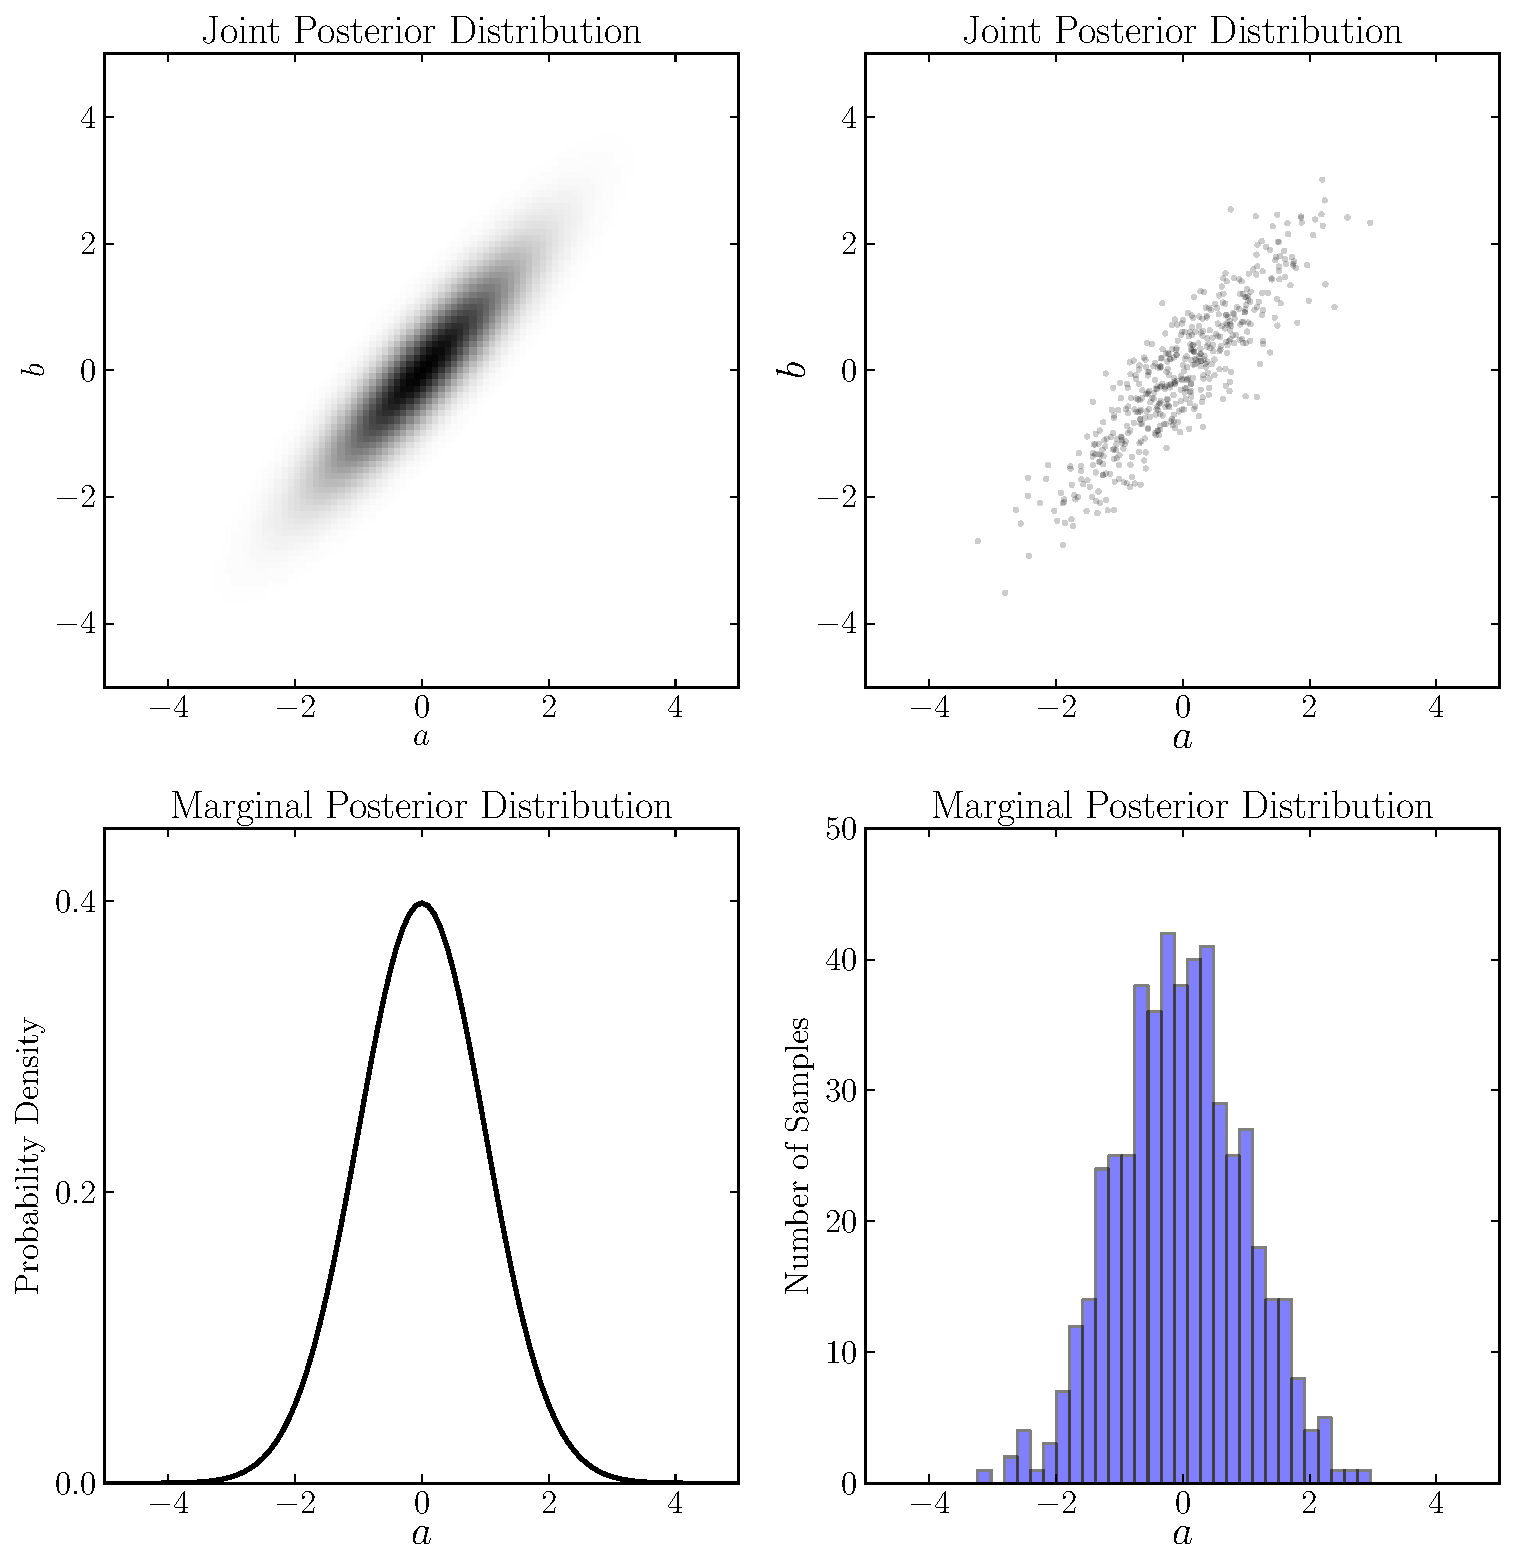
\includegraphics[scale=0.25]{marginalisation.pdf}
\end{column}

\end{columns}
\end{frame}

\begin{frame}[t]{Structure of the two example problems}
  \begin{itemize}
  \setlength{\itemsep}{10pt}
  \item There are $N$ objects in a region, and we don't know the value of $N$
  \item Each object has properties $\mathbf{x}_i$
  \item We have some data $\mathcal{D}$ which we want to use to infer both $N$
        and $\{\mathbf{x}_i\}_{i=1}^N$.
  \end{itemize}
\begin{center}
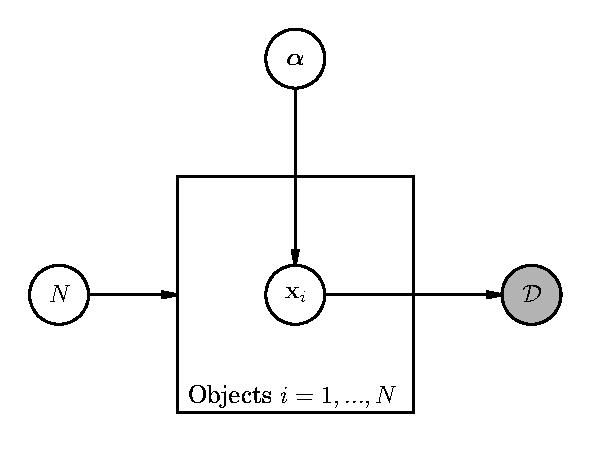
\includegraphics[scale=0.5]{../Paper/pgm.pdf}
\end{center}
\end{frame}

\begin{frame}[t]{Popular but slow approach}
The marginal posterior distribution for $N$ be written down directly
using Bayes' rule with $N$ as the only unknown parameter:
\begin{eqnarray}
p(N | D) &=& \frac{p(N)p(D | N)}{\sum_N p(N)p(D | N)}.
\end{eqnarray}
where
\begin{eqnarray}
p(D | N) &=& \int p(\theta | N) p(D | \theta, N) \, d^n \theta
\end{eqnarray}
\end{frame}

\begin{frame}[t]{Popular but slow approach}
Use many trial values of $N$ and use some Monte Carlo method to do the integral
for each $N$.
\end{frame}


\begin{frame}[t]{Alternative: Birth and Death}
For problems of unknown dimensionality, the hypothesis space is the union
of several fixed-dimension hypothesis spaces. Can add {\bf birth and death}
proposals that try to increase or decrease the number of objects in the model.

\begin{figure}
\begin{center}
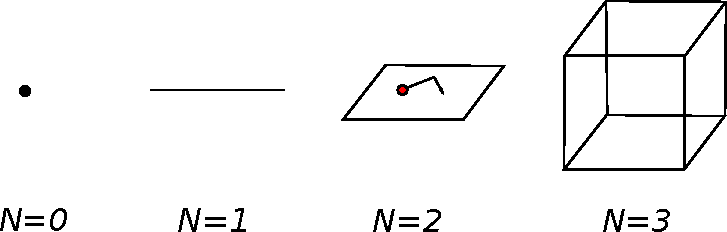
\includegraphics[scale=0.7]{drawing.pdf}
\end{center}
\end{figure}
\end{frame}


\begin{frame}[t]{Alternative: Birth and Death}
Birth and death moves are surprisingly easy to implement. Design them to
explore the prior (\& satisfy detailed balance), and then use
\begin{eqnarray}
\alpha = \min\left(1, \frac{p(D|\theta')}{p(D|\theta)}\right)
\end{eqnarray}
as the acceptance probability: i.e. just the ratio of likelihoods.
\end{frame}

\begin{frame}[t]{Alternative: Birth and Death}
Birth proposal: Increment $N$, generate the new 'object' from the prior
(given current values of hyperparameters)

\vspace{20pt}

Death proposal: Choose one of the $N$ objects, remove it, decrement $N$.
\end{frame}


\begin{frame}[t]{What's the issue?}
\begin{itemize}
\setlength{\itemsep}{20pt}
\item Birth-death MCMC seems to have solved our problem. Or has it?
\item What about these challenges?
\vspace{20pt}
  \begin{itemize}
  \setlength{\itemsep}{20pt}
  \item Multiple modes
  \item Strong degeneracies
  \item Phase transitions
  \end{itemize}
\end{itemize}
\end{frame}

\begin{frame}[t]{Challenging features}
\begin{center}
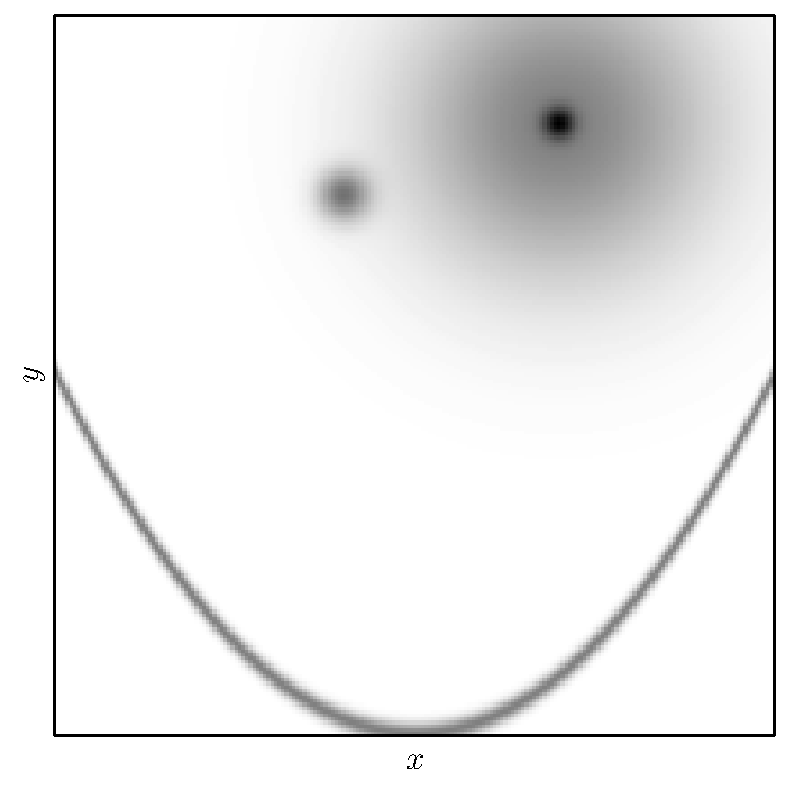
\includegraphics[scale=0.4]{challenges.pdf}
\end{center}
\end{frame}

\begin{frame}[t]{Nested Sampling}
In 2004, John Skilling introduced {\bf Nested Sampling}, a technique
that starts with the prior distribution, and shrinks volume at a controlled
rate.
\vspace{20pt}

{\bf Nested Sampling solves the problem of phase transitions and (as far as I
know) no other Monte Carlo method does.}
\end{frame}

\begin{frame}[t]{Diffusive Nested Sampling}
\begin{columns}[T]
\begin{column}{0.35\textwidth}
  \vspace{10pt}
  \begin{itemize}
  \setlength{\itemsep}{20pt}
  \item Replace the posterior distribution with a {\bf mixture of constrained priors}
  \item Can cross valleys (the prior is a mixture component)
  \item Posterior is available via re-weighting
  \end{itemize}
\end{column}
\hfill
\begin{column}{0.5\textwidth}
  \hspace{50pt}
  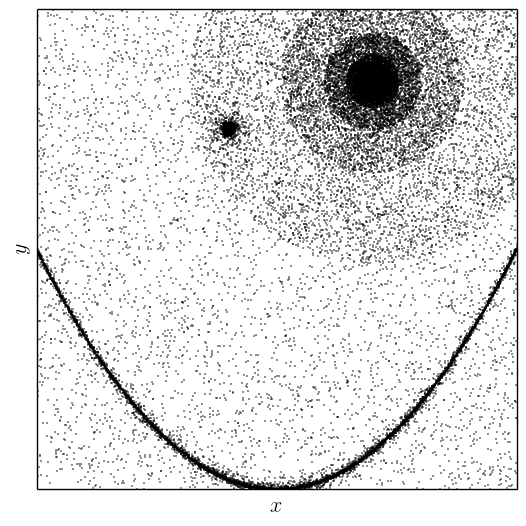
\includegraphics[scale=0.4]{dnest.png}
\end{column}
\end{columns}
\end{frame}

\begin{frame}[t]{Diffusive Nested Sampling}
\begin{itemize}
\setlength{\itemsep}{20pt}
\item I've implemented a library, {\tt RJObject}, that handles all the
Metropolis proposals I need for these kinds of problems.
\item Uses birth-death MCMC, but exploring the DNS distribution, rather than
the (harder) posterior.
\end{itemize}
\end{frame}

\begin{frame}[t]{Motivating Problem I}
\begin{itemize}
\item How many sinusoids are in this data?
\item Also, what are their periods, amplitudes and phases?
\end{itemize}
\begin{center}
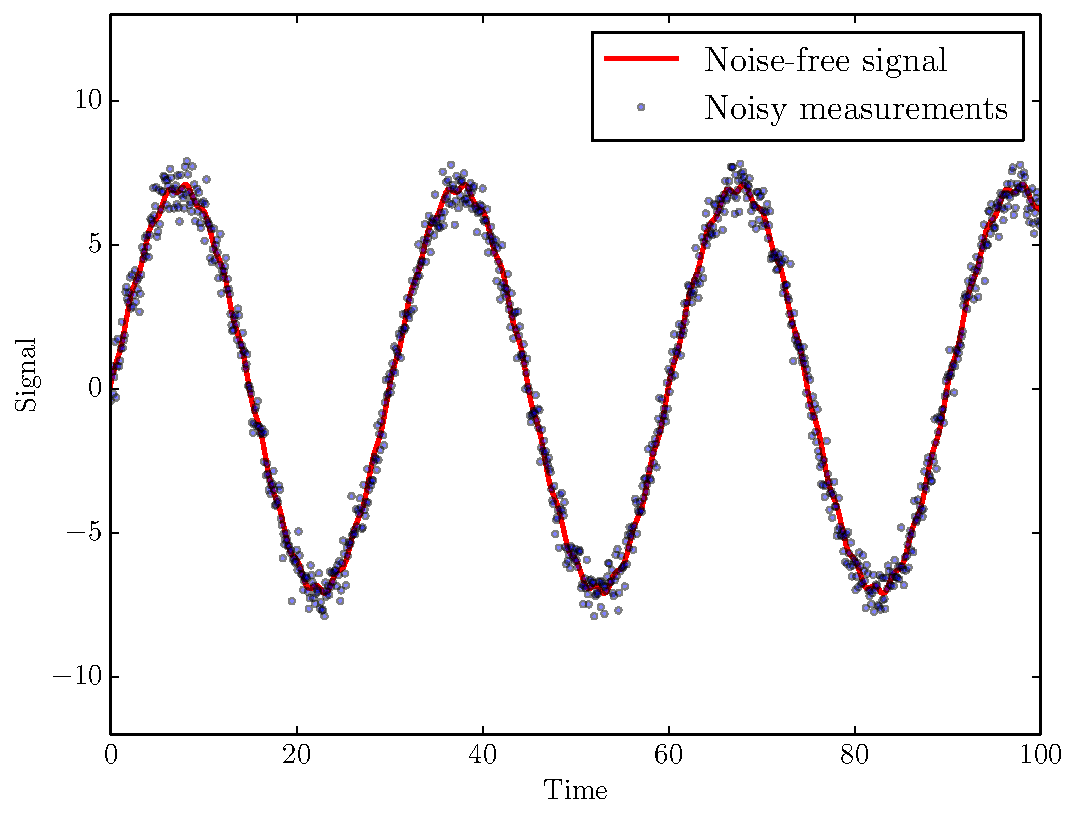
\includegraphics[scale=0.35]{sinewave_data.pdf}
\end{center}
\end{frame}

\begin{frame}[t]{Results from the sinusoid data}
The $N=1$ and $N=2$ solutions are separated by a phase transition.
\begin{center}
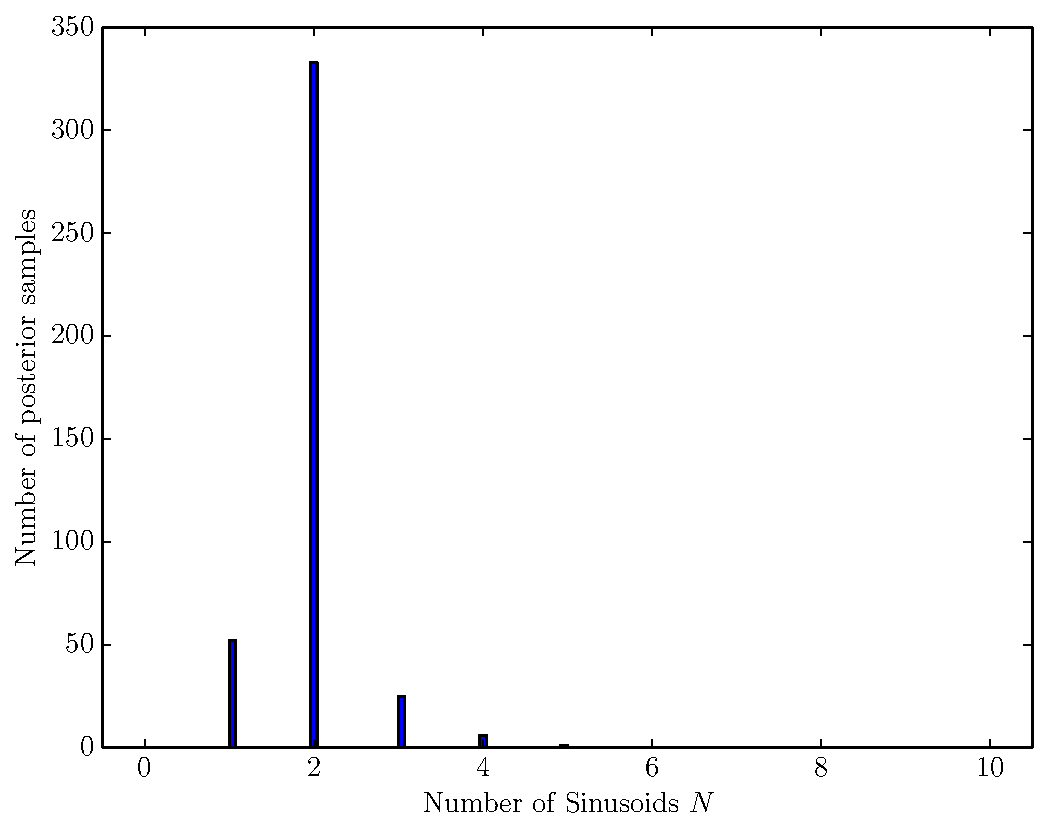
\includegraphics[scale=0.45]{../Paper/N_result.pdf}
\end{center}
\end{frame}

\begin{frame}[t]{Sinusoid data movie}
{\tt https://www.youtube.com/watch?v=i-f4VqPPeGg}
\end{frame}

\begin{frame}[t]{Motivating Problem II}
\begin{itemize}
\item How many stars are in these images?
\item Also, what are their positions, fluxes, etc?
\end{itemize}
\begin{center}
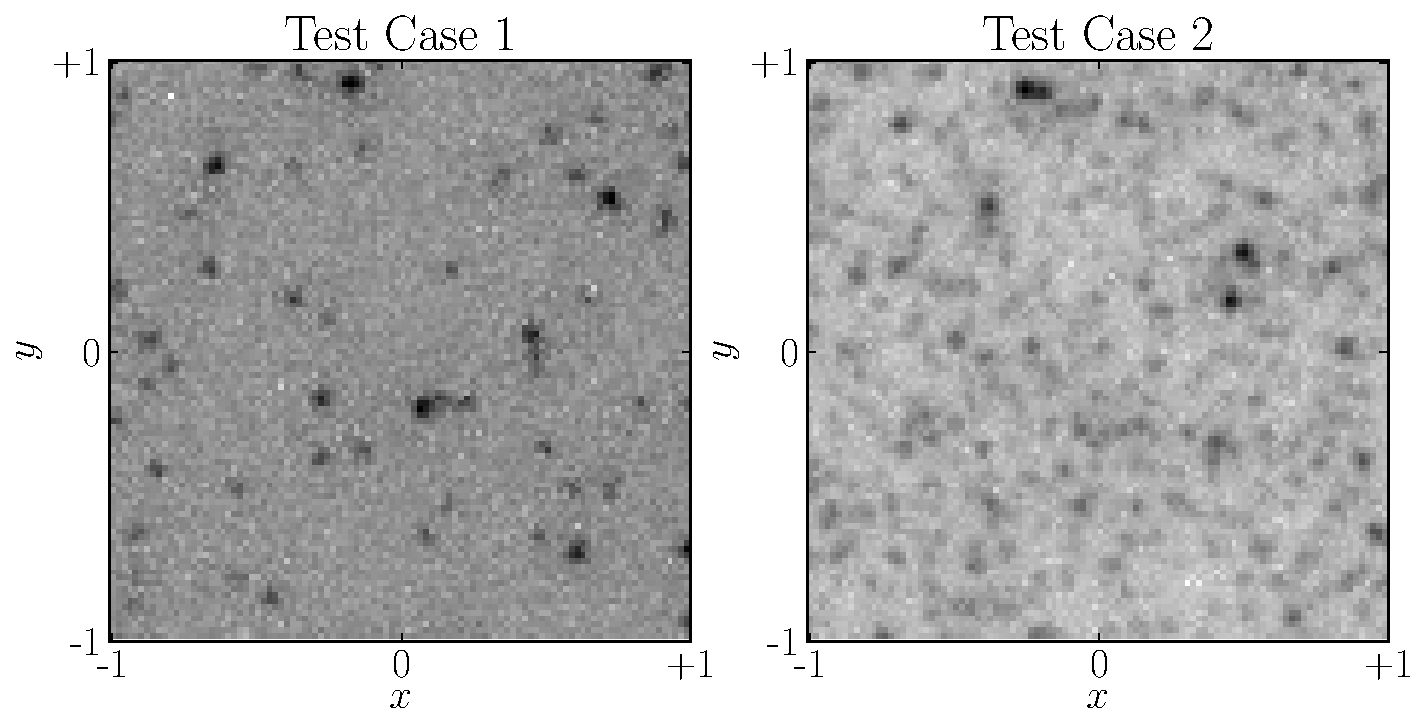
\includegraphics[scale=0.35]{test_cases.pdf}
\end{center}
\end{frame}

\begin{frame}[t]{Probabilistic catalogs}
\begin{center}
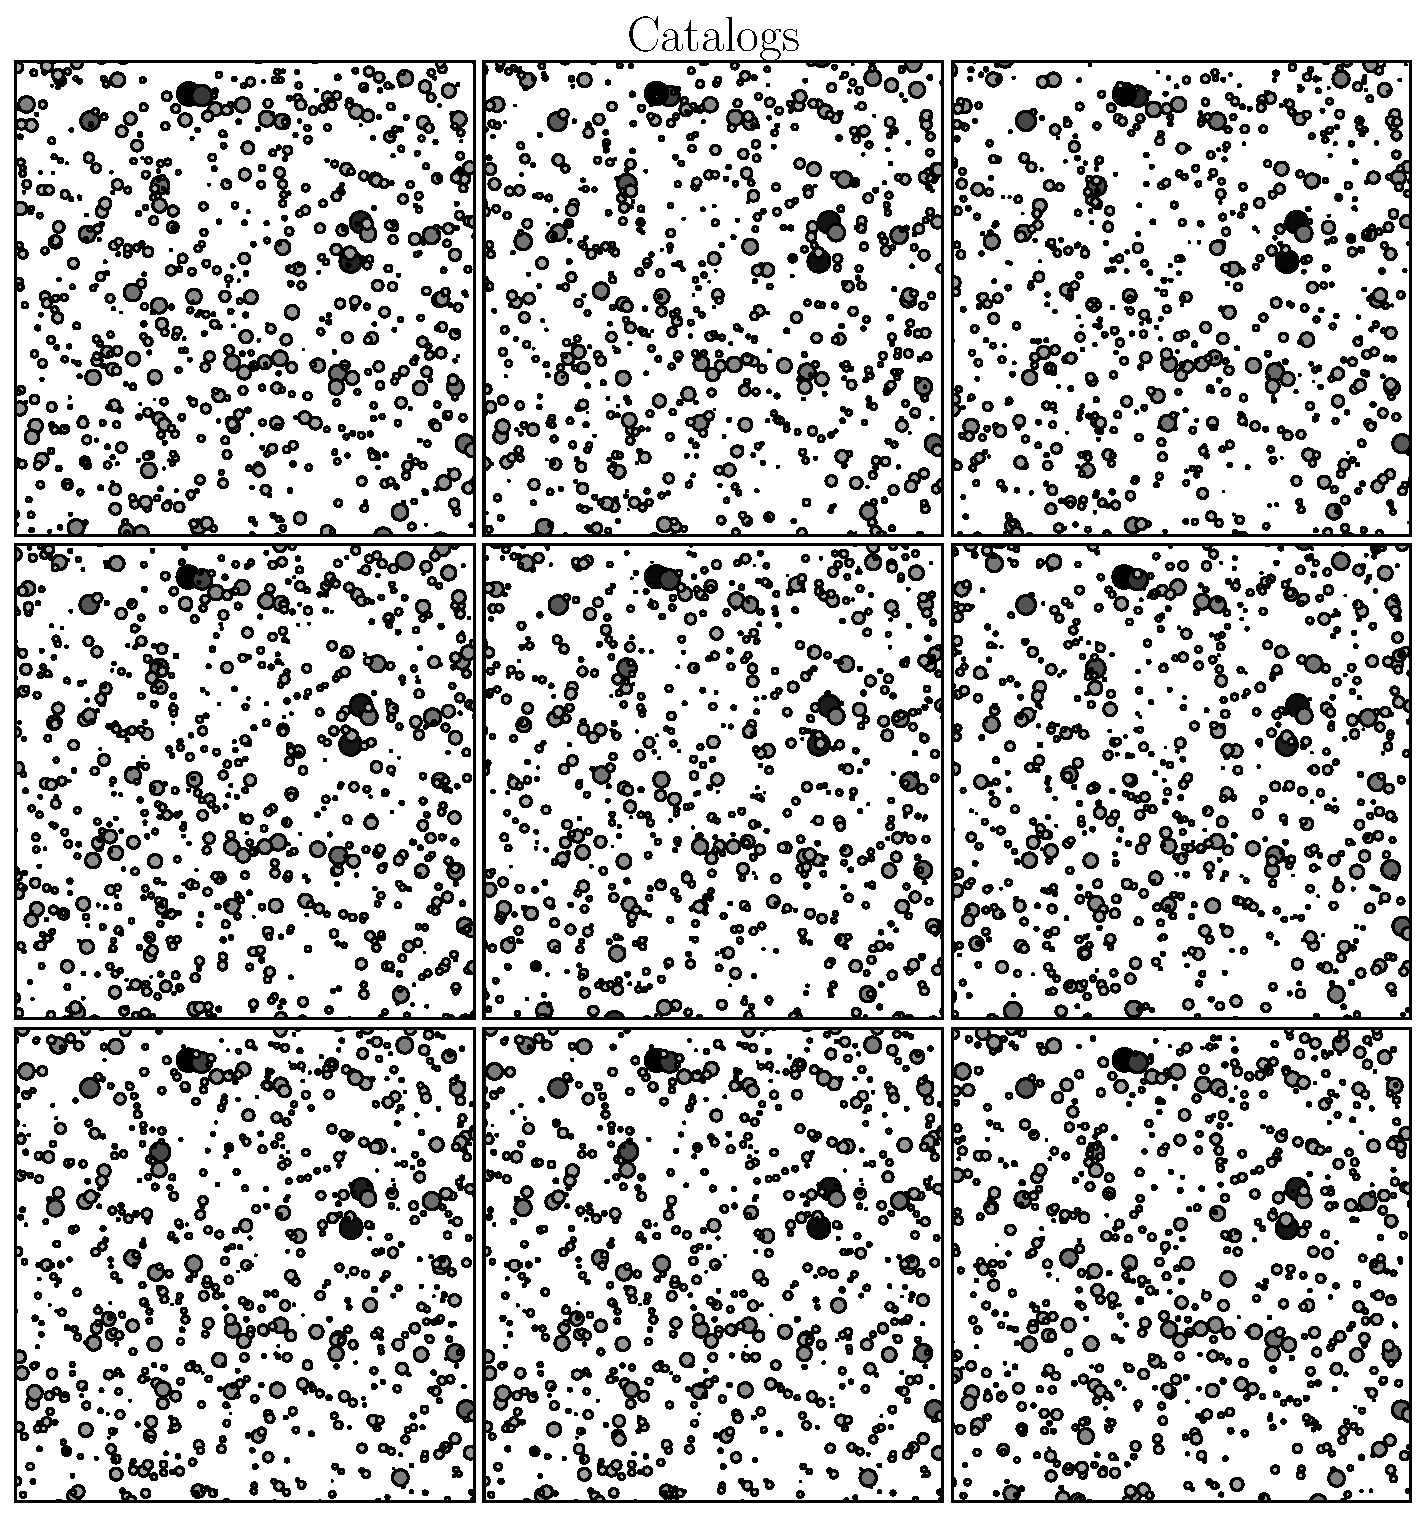
\includegraphics[scale=0.25]{StarFieldFigures/catalogs.pdf}
\end{center}
\end{frame}

\begin{frame}[t]{Hyperparameters}
\begin{center}
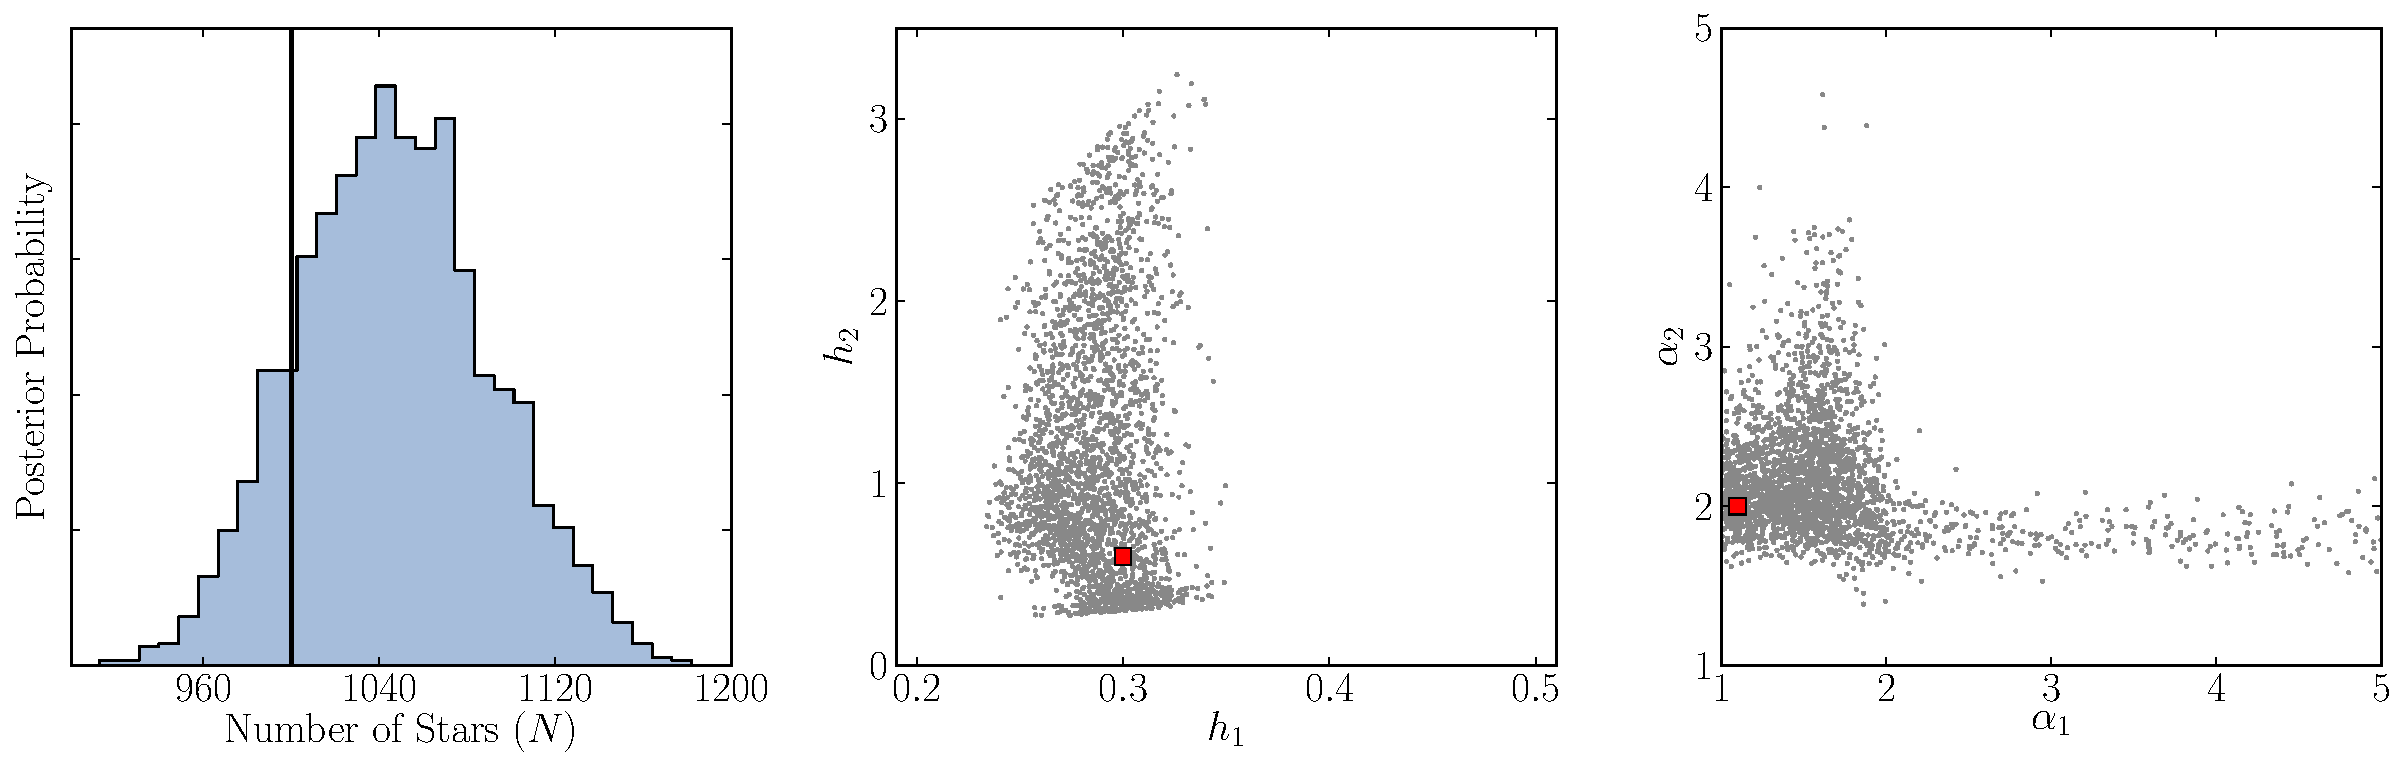
\includegraphics[scale=0.28]{StarFieldFigures/inference2.pdf}
\end{center}
\end{frame}

\begin{frame}[t]{Luminosity Function}
\begin{center}
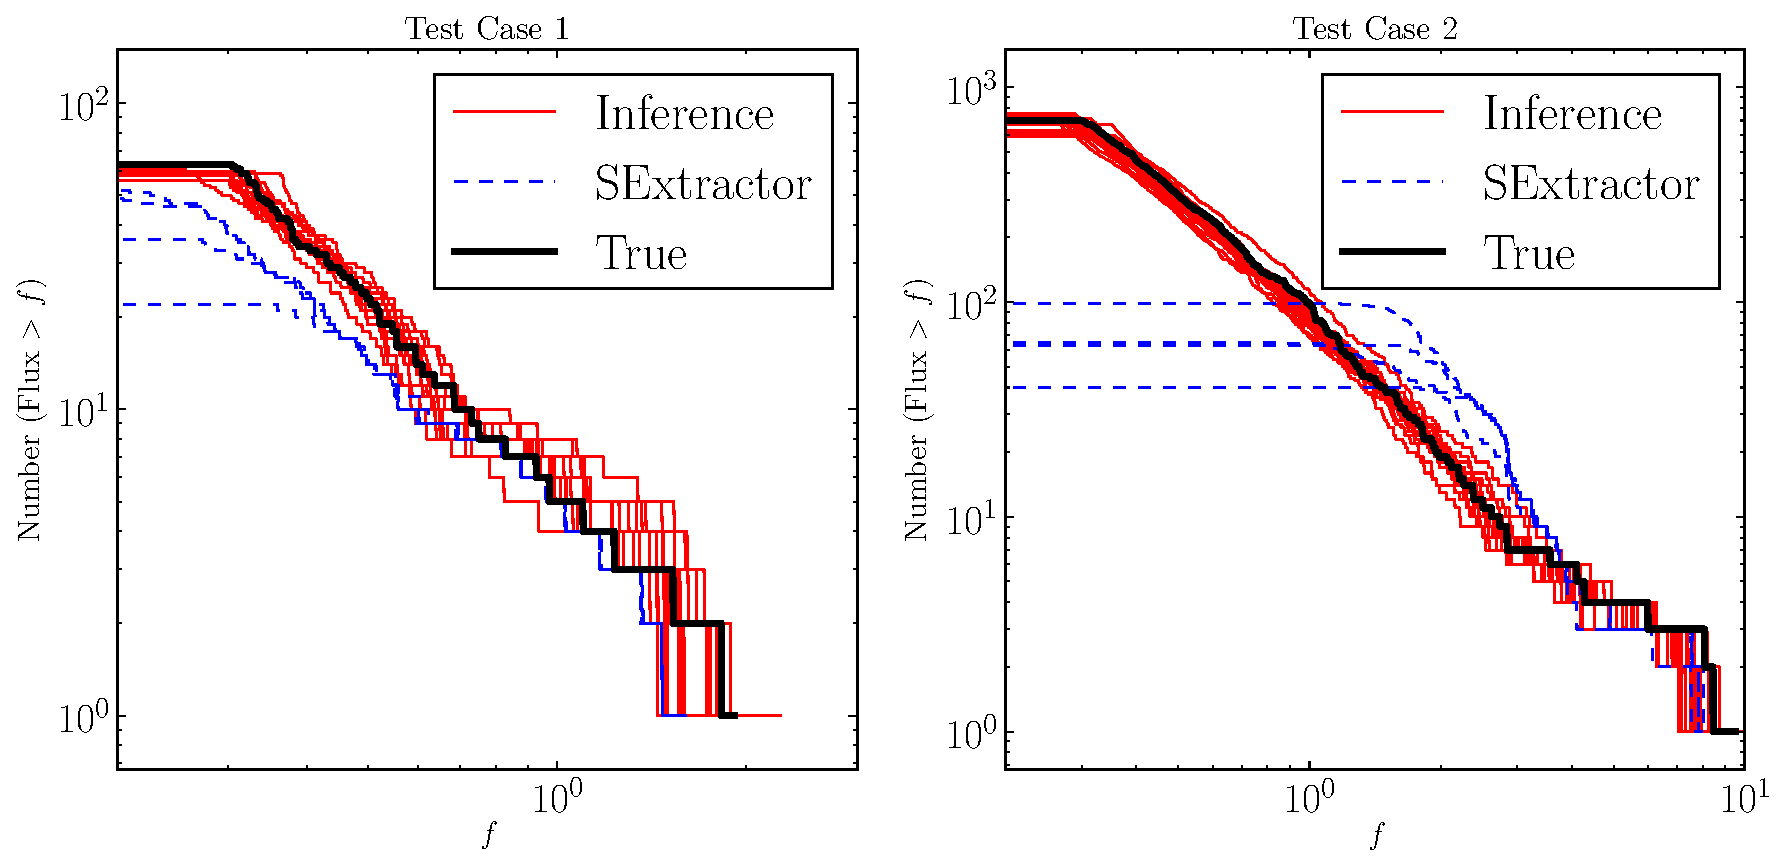
\includegraphics[scale=0.35]{StarFieldFigures/luminosity_function.pdf}
\end{center}
\end{frame}

\begin{frame}[t]{Recommendations}
It is infeasible to apply this approach wholesale.
Instead I would use it on small subsets of imaging that are of specific interest.

\vspace{20pt}

\begin{center}
{\it Any takers?}
\end{center}
\end{frame}



\begin{frame}[t]{Exoplanets}
Radial velocity data is considered challenging. There are many systems where
controversy rages over $N$.
\end{frame}

\begin{frame}[t]{Exoplanets: Simulated Dataset}
How many planets?
\begin{center}
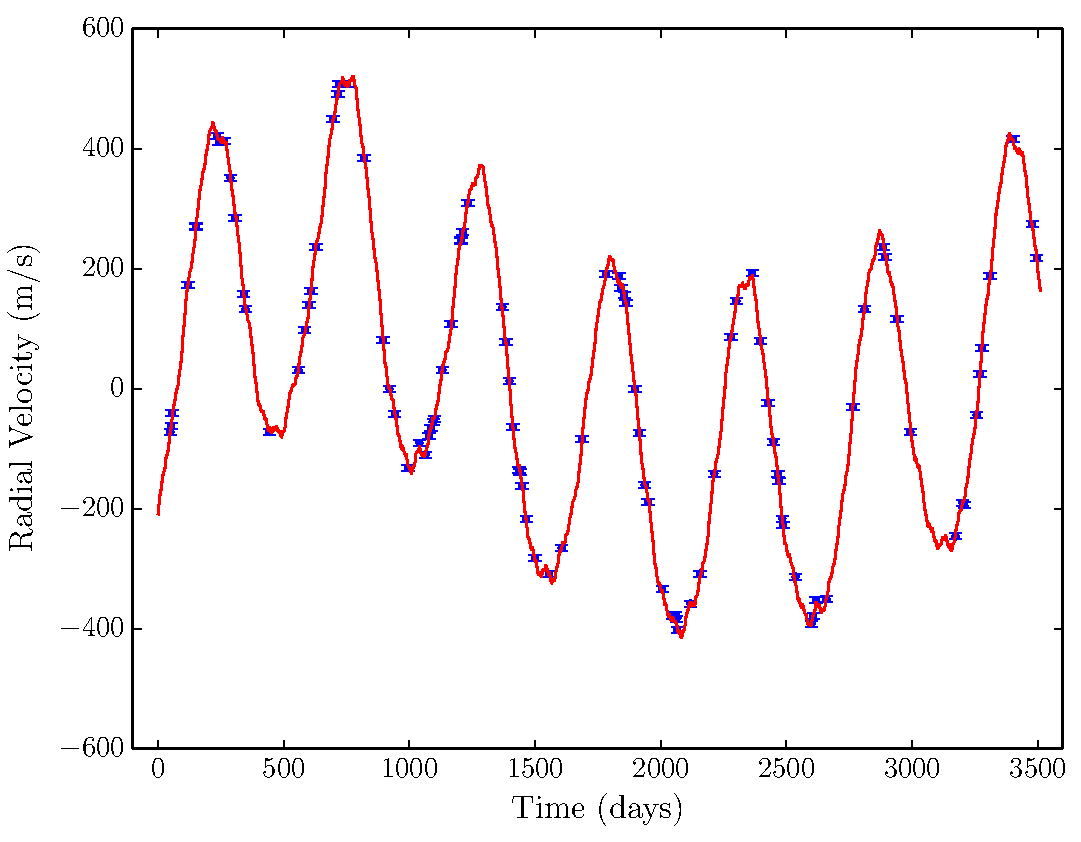
\includegraphics[scale=0.35]{ExoplanetFigures/fake_data.pdf}
\end{center}
\end{frame}

\begin{frame}[t]{Exoplanets: Simulated Dataset Results}
The true value was $N$=7.
\begin{center}
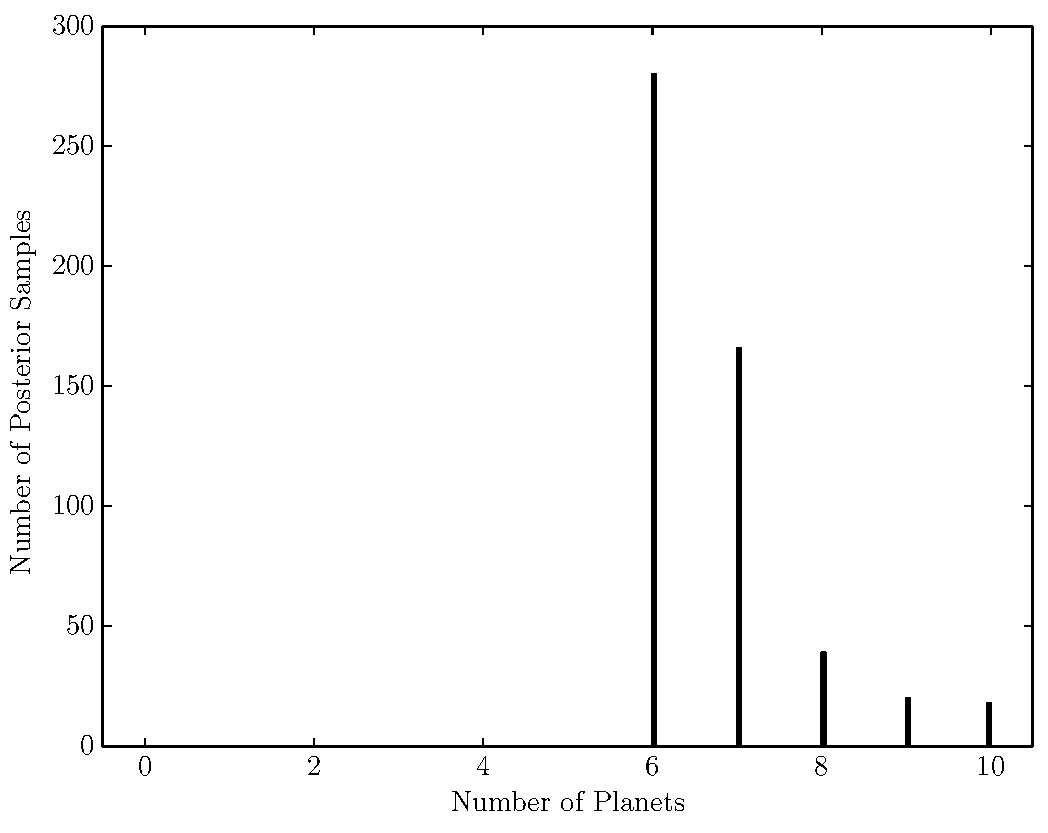
\includegraphics[scale=0.35]{ExoplanetFigures/fake_data_N.pdf}
\end{center}
\end{frame}

\begin{frame}[t]{Exoplanets: Simulated Dataset Results}
This is the posterior distribution for $P_1$. Keep in mind the {\bf
label-switching degeneracy}.
\begin{center}
\includegraphics[scale=0.35]{ExoplanetFigures/fake_data_periods.pdf}
\end{center}
\end{frame}

\begin{frame}[t]{Exoplanets: Simulated Dataset Results}
Here, we can see why one of the planets was not ``detected'':
\begin{center}
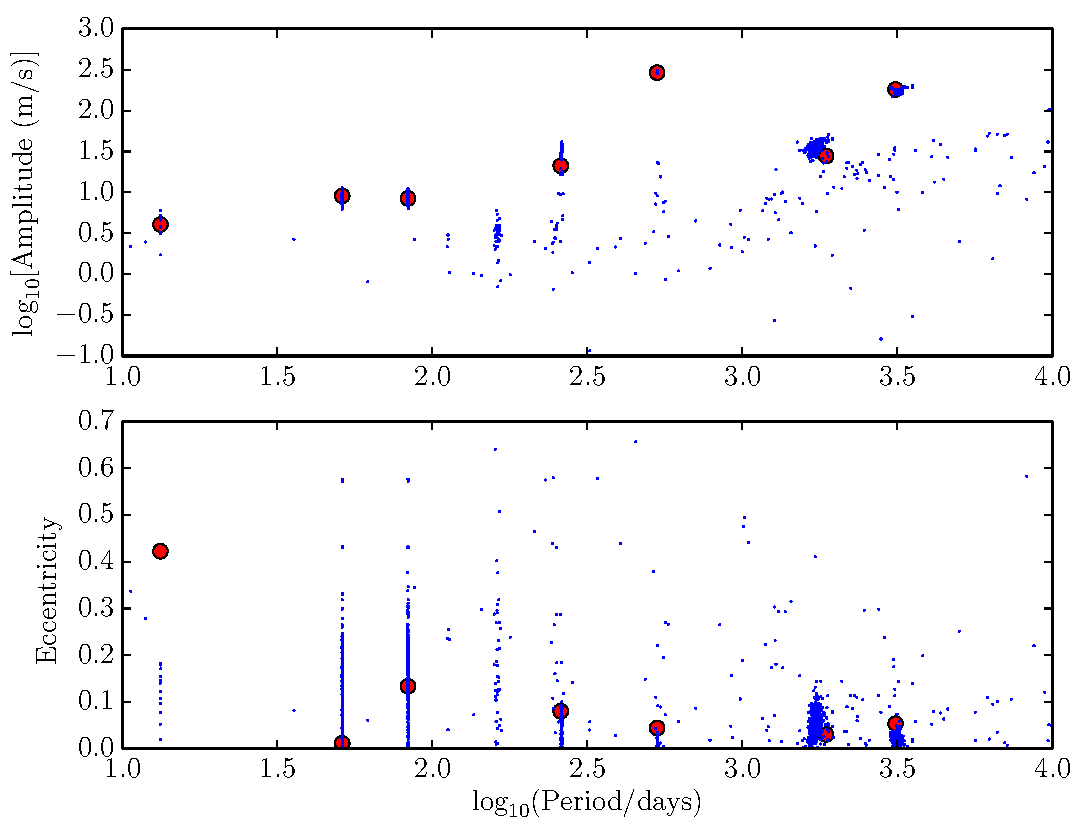
\includegraphics[scale=0.35]{ExoplanetFigures/fake_data_posterior.pdf}
\end{center}
\end{frame}

\begin{frame}[t]{Time}
It takes about 15-20 minutes to obtain some posterior samples.

Compare with Phil Gregory's code (30 minutes per planet, no trans dimensional
moves).
\end{frame}

\begin{frame}[t]{Gliese 581}
Gliese 581 is an M dwarf which has been observed extensively with the HARPS
and UVES spectrographs.

\vspace{20pt}

There is controversy about $N$, some people only
believe {\bf two} of the claimed planets, while other analyses suggest
{\bf up to 6} (with a few of these in the habitable zone).
\end{frame}

\begin{frame}[t]{Giant Disclaimer}
\begin{center}
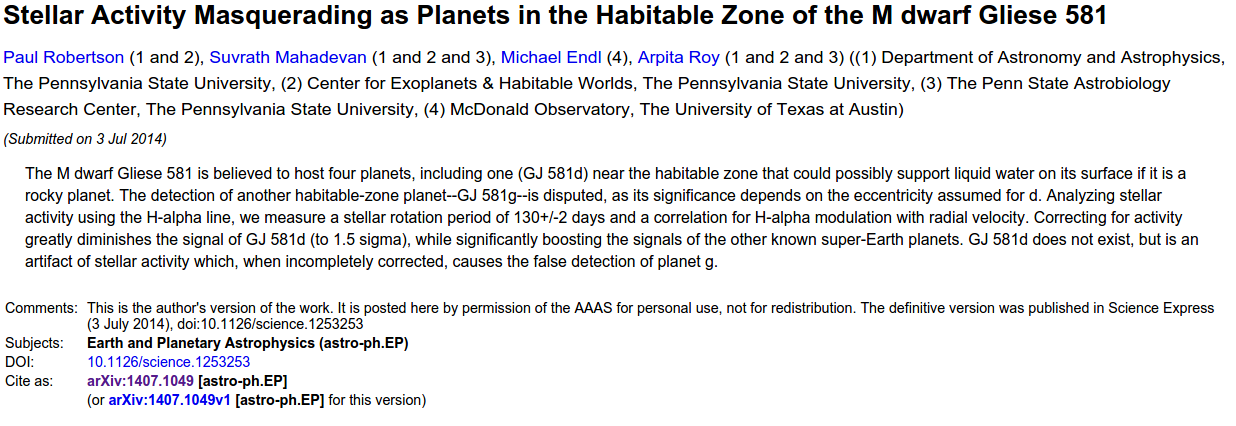
\includegraphics[scale=0.25]{robertson.png}
\end{center}
\end{frame}

\begin{frame}[t]{Giant Disclaimer}
\begin{center}
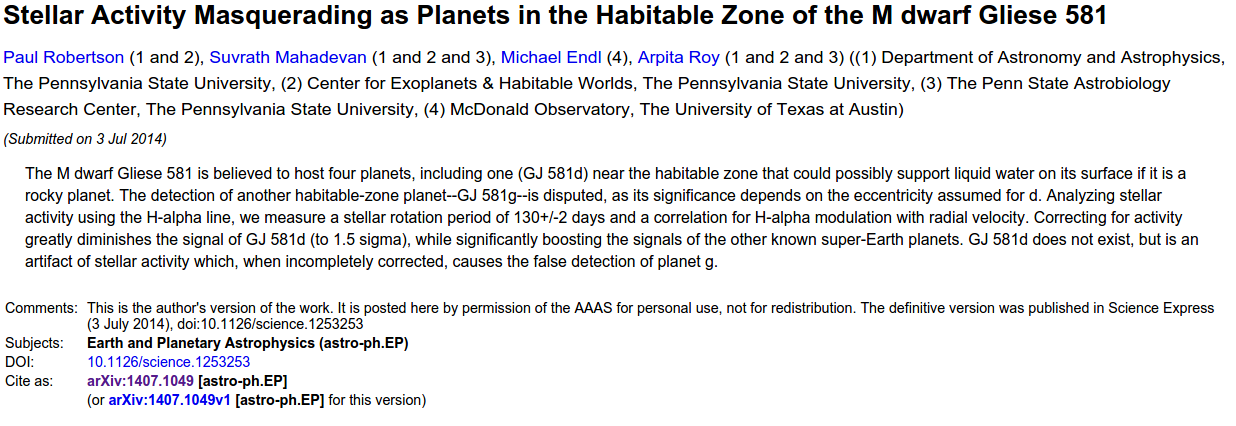
\includegraphics[scale=0.25]{robertson.png}
\end{center}
\end{frame}



\begin{frame}[t]{Real projects}
\begin{itemize}
\item Magnetar bursts
\item Making probabilistic catalogs
\item Gravitational lens time delays in unresolved systems
\item Gravitational lens inversion
\item Modelling the progress of parallel Nested Sampling runs (!)
\end{itemize}
\end{frame}

\begin{frame}[t]{Software}
\begin{itemize}
\setlength{\itemsep}{20pt}
\item Diffusive Nested Sampling in C++
{\tt github.com/eggplantbren/DNest3}
\item Birth-death models in C++
{\tt github.com/eggplantbren/RJObject}
\item These are free software (GPLd).
\item The learning curve is steep (sorry) but I'm open to collaborations.
\end{itemize}
\end{frame}

